\documentclass[11pt]{article}
    %	options include 12pt or 11pt or 10pt
    %	classes include article, report, book, letter, thesis
    
    \title{HW4}
    \author{Shane Drafahl}
    \date{18 September ,2017}
    \usepackage{graphicx}
    \usepackage{epstopdf}
    \usepackage{graphics}

    \begin{document}
    \maketitle

    1. Let $ |x|_{a} $ be the number of occurrences of the symbol a in the string x.

    $ \newline $

    Define a context-free grammar for the language $ L = \{\ w \in \{\ 1, 0 \}\ ^{*} : |w|_{0} = |w|_{1} \}\ $

    $ \newline \newline $

    G = $ \{\ (S), (1,0), S, P  \}\ $
    $ \newline $
    $ P = \{\ $ 
    $ S \rightarrow 01 | 10 | 1S0 | 0S1 | SSS | \epsilon $
    $ \}\ $

    $ \newline $

    Using a inductive proof I will give a formal proof that the grammar genderate L

    $ \newline $

    Basis: $ 01 \in \{\ 1, 0 \}\ ^{*} , 10 \in \{\ 1, 0 \}\ ^{*} and \epsilon \in \{\ 1, 0 \}\ ^{*} $
    and for all cases there are either one 1 and one 0 or zero 0 and zero 1.
    $ \newline $

    IH: Suppose that $ w $ can be generated from G and that $ w \in L $

    $ \newline $

    Structural: Suppose that there are strings A,B,C and $ A,B,C \in L $ by the IH and they are all generated from G. Suppose 
    that they are concatenated ABC or CBA. All strings have the same number of 1's and 0's so therefore the resulting 
    string ABC or CBA would also have have the same number of 1's and 0's so $ ABC, CBA \in L $. One of the transitions 
    in the grammar is $ S \rightarrow SSS $ so $ S \rightarrow ABC $ or $ S \rightarrow CBA $ since we know from the IH that
    $ A,B,C \in L $ so therefore $ S \rightarrow A,B,C $. Therefore ABC and CBA can be created by the grammar G and they are in 
    the language L.

    $ \newline $

    2. Define a NPDA for the language $ L = \{\ a^{n}b^{m} : m,n \in N, m \leq n \leq 2m \}\ $

    $ \newline $

    

    $ \newline $

    3. 

    $ \newline $

        \begin{figure}[!htb]
            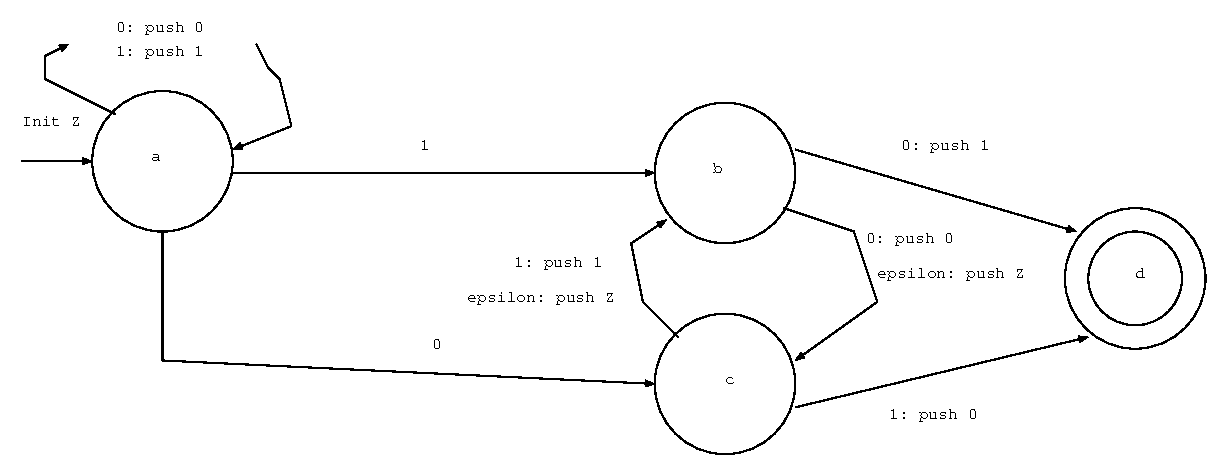
\includegraphics[scale=.7]{./hw7.eps}
        \end{figure}
    


    \end{document}